\documentclass[journal,12pt,twocolumn]{IEEEtran}

\usepackage{setspace}
\usepackage{gensymb}
\singlespacing
\usepackage[cmex10]{amsmath}

\usepackage{amsthm}

\usepackage{mathrsfs}
\usepackage{txfonts}
\usepackage{stfloats}
\usepackage{bm}
\usepackage{cite}
\usepackage{cases}
\usepackage{subfig}

\usepackage{longtable}
\usepackage{multirow}
\usepackage{enumitem}
\usepackage{mathtools}
\usepackage{steinmetz}
\usepackage{tikz}
\usepackage{circuitikz}
\usepackage{verbatim}
\usepackage{tfrupee}
\usepackage[breaklinks=true]{hyperref}
\usepackage{graphicx}
\usepackage{tkz-euclide}

\usetikzlibrary{calc,math}
\usepackage{listings}
    \usepackage{color}                                            %%
    \usepackage{array}                                            %%
    \usepackage{longtable}                                        %%
    \usepackage{calc}                                             %%
    \usepackage{multirow}                                         %%
    \usepackage{hhline}                                           %%
    \usepackage{ifthen}                                           %%
    \usepackage{lscape}     
\usepackage{multicol}
\usepackage{chngcntr}

\DeclareMathOperator*{\Res}{Res}

\renewcommand\thesection{\arabic{section}}
\renewcommand\thesubsection{\thesection.\arabic{subsection}}
\renewcommand\thesubsubsection{\thesubsection.\arabic{subsubsection}}

\renewcommand\thesectiondis{\arabic{section}}
\renewcommand\thesubsectiondis{\thesectiondis.\arabic{subsection}}
\renewcommand\thesubsubsectiondis{\thesubsectiondis.\arabic{sub subsection}}


\hyphenation{optical networks semiconduc-tor}
\def\inputGnumericTable{}                                 %%

\lstset{
%language=C,
frame=single, 
breaklines=true,
columns=fullflexible
}
\date{March 2021}

\begin{document}

\newcommand{\BEQA}{\begin{eqnarray}}
\newcommand{\EEQA}{\end{eqnarray}}
\newcommand{\define}{\stackrel{\triangle}{=}}
\bibliographystyle{IEEEtran}
\raggedbottom
\setlength{\parindent}{0pt}
\providecommand{\mbf}{\mathbf}
\providecommand{\pr}[1]{\ensuremath{\Pr\left(#1\right)}}
\providecommand{\qfunc}[1]{\ensuremath{Q\left(#1\right)}}
\providecommand{\fn}[1]{\ensuremath{f\left(#1\right)}}
\providecommand{\e}[1]{\ensuremath{E\left(#1\right)}}
\providecommand{\sbrak}[1]{\ensuremath{{}\left[#1\right]}}
\providecommand{\lsbrak}[1]{\ensuremath{{}\left[#1\right.}}
\providecommand{\rsbrak}[1]{\ensuremath{{}\left.#1\right]}}
\providecommand{\brak}[1]{\ensuremath{\left(#1\right)}}
\providecommand{\lbrak}[1]{\ensuremath{\left(#1\right.}}
\providecommand{\rbrak}[1]{\ensuremath{\left.#1\right)}}
\providecommand{\cbrak}[1]{\ensuremath{\left\{#1\right\}}}
\providecommand{\lcbrak}[1]{\ensuremath{\left\{#1\right.}}
\providecommand{\rcbrak}[1]{\ensuremath{\left.#1\right\}}}
\theoremstyle{remark}
\newtheorem{rem}{Remark}
\newcommand{\sgn}{\mathop{\mathrm{sgn}}}
\providecommand{\abs}[1]{\vert#1\vert}
\providecommand{\res}[1]{\Res\displaylimits_{#1}} 
\providecommand{\norm}[1]{\lVert#1\rVert}
%\providecommand{\norm}[1]{\lVert#1\rVert}
\providecommand{\mtx}[1]{\mathbf{#1}}
\providecommand{\mean}[1]{E[ #1 ]}
\providecommand{\fourier}{\overset{\mathcal{F}}{ \rightleftharpoons}}
%\providecommand{\hilbert}{\overset{\mathcal{H}}{ \rightleftharpoons}}
\providecommand{\system}{\overset{\mathcal{H}}{ \longleftrightarrow}}
	%\newcommand{\solution}[2]{\textbf{Solution:}{#1}}
\newcommand{\solution}{\noindent \textbf{Solution: }}
\newcommand{\cosec}{\,\text{cosec}\,}
\providecommand{\dec}[2]{\ensuremath{\overset{#1}{\underset{#2}{\gtrless}}}}
\newcommand{\myvec}[1]{\ensuremath{\begin{pmatrix}#1\end{pmatrix}}}
\newcommand{\mydet}[1]{\ensuremath{\begin{vmatrix}#1\end{vmatrix}}}
\numberwithin{equation}{subsection}
\makeatletter
\vspace{3cm}
\title{Assignment 4}
\author{Adhvik Mani Sai Murarisetty - AI20BTECH11015}
\maketitle
\newpage
\bigskip
\renewcommand{\thetable}{\theenumi}
Download all python codes from 
\begin{lstlisting}
https://github.com/adhvik24/AI1103-PROBABILITY-AND-RANDOM-VARIABLES/tree/main/ASSIGNMENT_4/codes
\end{lstlisting}
%
and latex-tikz codes from 
%
\begin{lstlisting}
https://github.com/adhvik24/AI1103-PROBABILITY-AND-RANDOM-VARIABLES/tree/main/ASSIGNMENT_4/AI1103_Assignment4.tex
\end{lstlisting}
\section{GATE 2016 (XE-A),Q.8 (Engg. Maths section)}
A diagnostic test for a certain disease is 90\% accurate. That is, the probability of a person having (respectively, not having) the disease tested positive (respectively, negative) is 0.9. Fifty percent of the population has the disease. What is the probability that a randomly chosen person has the disease given that the person tested negative?
\section{SOLUTION}
Let X and Y be two Bernoulli random variables such that X,Y$\in$\cbrak{0,1} and as given fifty percent of the population has the disease, the probability mass function of X is 
\begin{align}
    p_{X}(n) = \pr{X = n} = 
\begin{cases}
0.5 &  n=1
\\
0.5 & n=0
\\
0 & otherwise
\end{cases}\label{1}
\end{align}
where X denotes the health status of a person(X=1 if person is healthy and X=0 if person is diseased) and Y denotes the diagnostic test result (Y=1 if it is positive and Y=0 if it is negative).
\\Given the probabilities of,
\begin{align}
    \pr{Y=1|X=0}=0.9\label{2}
    \\\pr{Y=0|X=1}=0.9 \label{3}
\end{align}
we need to find $\pr{X=0|Y=0}$,
\begin{align}
    \pr{X=0|Y=0}&=\frac{\pr{X=0\cap Y=0}}{\pr{Y=0}}\\
    \pr{X=0|Y=0}&=\frac{\pr{Y=0|X=0}\pr{X=0}}{\pr{Y=0}}\label{4}
\end{align}
\begin{multline}
    \pr{Y=0}=\pr{Y=0|X=1}\pr{X=1}\\+\pr{Y=0|X=0}\pr{X=0}\label{5}
\end{multline}
Using \eqref{1},\eqref{2} and \eqref{3} in \eqref{5},
\begin{align}
    \nonumber\pr{Y=0}&=0.9(0.5)+(1-0.9)0.5\\
    \pr{Y=0}&= 0.5\label{6}
\end{align}
Using \eqref{1},\eqref{2} and \eqref{6} in \eqref{4}
\begin{align}
    \pr{X=0|Y=0}&=\frac{(1-0.9)0.5}{0.5}\\
    \pr{X=0|Y=0}&= 0.1
\end{align}
\begin{figure}[htp]
    \centering
    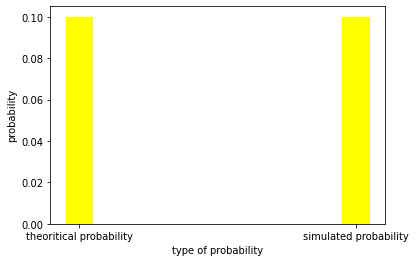
\includegraphics[width=\columnwidth]{assign4.png}
    \caption{probability that a randomly chosen person has the disease given that the person tested negative }
\end{figure}

Therefore the probability that a randomly chosen person has the disease given that the person tested negative is 0.1.
\end{document}
